% !TeX root = ../tfm.tex
%! TEX root = ../tfm.tex

Estudiaremos los resultados obtenidos por los desarrollos de este trabajo en dos bloques. En el primero analizaremos el algoritmo y modelos generados frente al estado del arte en modelos de detección de caídas y evaluaremos el grado de satisfacción de las metas deseadas. En segunda instancia introduciremos los resultados obtenidos con la aplicación \ifell/. Estudiaremos la viabilidad del acercamiento propuesto desde a nivel técnico y funcional así como la adecuación a solventar el problema y metas a lograr.

\section{Evaluación del modelo y algoritmo de \ifell/}

Un sistema de detección de caídas es en el fondo un clasificador con una única clase. Todos los resultados pueden por tanto agruparse en los que pertenecen o no a dicho conjunto. Con el fin de evaluar y comparar los resultados obtenidos usaremos dos métricas estadísticas:
\begin{itemize}
  \item Sensitividad (Capacidad de identificar las caídas), también conocida como \textit{recall}.
  \[
    Sensitividad = \frac{TP}{TP+FN}
  \]
  \item Especificidad o Selectividad (Capacidad de discernir únicamente las caídas).
  \[
    Especificidad = \frac{TN}{TN+FP}
  \]
\end{itemize}

Finalmente, como criterio de evaluación promediado de ambas en este trabajo hemos usado un promediado ponderado que daba mayor importancia a la sensibilidad sobre la especificidad pues tenemos como exigencia lograr un clasificador con la mayor sensibilidad posible. Sin embargo de cara a la evaluación usaremos la \textit{exactitud promediada} definida como:\[
  ExactitudPromediada=\frac{Sensibilidad+Especificidad}{2}
\]

Estas métricas son usadas habitualmente en otros trabajos similares\cite{Noury2007,Chen2005, Bourke2006} y permite utilizar los mismos indicadores para analizar los resultados de diferentes modelos directamente.

\subsection{Evaluación del algoritmo sobre SisFall}\label{sub:eval:hibrido}

\subsubsection{Metodología}

Partiendo del algoritmo de \ifell/ descrito en en \fullref{sec:imp:model}, usaremos un detector \textit{BourkeU} con cota de decisión fijada a 5g como modelo analítico y los modelos \textit{RNN-R(175)[50]}, \textit{RNN-P(175)[50]} y \textit{RNN-R(350)[50]} para el bloque de decisión final. Analizaremos los resultados para varios valores de la cota de decisión sobre el RMSE así como de la posición del punto de impacto $t_0$.

Recuperamos las mismas particiones de \sisfall/ hechas para el entrenamiento de los modelos que recordemos estaban conformadas con un 80\% para entrenamiento y el 20\% de muestras para validación. De la misma forma que analizamos el comportamiento del algoritmo de Bourke en la sección \ref{sub:imp:model:analitico} observaremos el comportamiento del algoritmo de modelo híbrido de \ifell/. Usando el subconjunto de entrenamiento para definir la cota de decisión sobre el error RMSE se la salida del modelo codificador/decodificador con la señal esperada y posteriormente evaluaremos los resultados obtenidos tras aplicar el algoritmo al conjunto de validación en relación a la literatura existente.

\subsubsection{Obtención de la cota del RMSE de decisión}

Alimentamos las tres variaciones elegidas con las sesiones del conjunto de validación y calculamos el RMSE para cada ejercicio de la base de datos. Almacenamos el resultado para poder calcular el histograma de manera similar a como hicimos con el modelo de Bourke.

\begin{figure}[!ht]
  \centering
  \begin{subfigure}[b]{0.31\textwidth}
      \centering
      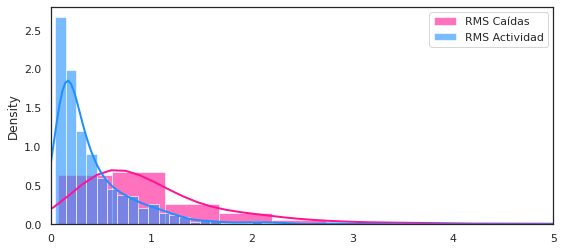
\includegraphics[width=\linewidth]{SISFALL175_RECON_RMS_HIST.png}
      \caption{\footnotesize \label{fig:ifell:sisfall:rmshist:175:recon}Distribuciones de RMSE para actividades y caídas en el modelo RNN-R(175)[50]}
  \end{subfigure}
  \hfill
  \begin{subfigure}[b]{0.31\textwidth}
      \centering
      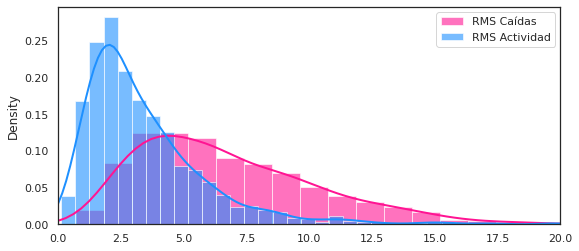
\includegraphics[width=\linewidth]{SISFALL175_PRED_RMS_HIST.png}
      \caption{\footnotesize \label{fig:ifell:sisfall:rmshisit:175:pred}Distribuciones de RMSE para actividades y caídas en el modelo RNN-P(175)[50]}
  \end{subfigure}
  \hfill
  \begin{subfigure}[b]{0.31\textwidth}
      \centering
      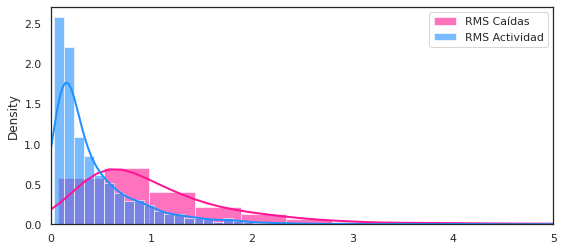
\includegraphics[width=\linewidth]{SISFALL350_RECON_RMS_HIST.png}
      \caption{\footnotesize \label{fig:ifell:sisfall:rmshist:350:pred}Distribuciones de RMSE para actividades y caídas en el modelo RNN-R(350)[50]}
  \end{subfigure}
  \caption{\footnotesize \label{fig:ifell:sisfall:rmshist}Histogramas del RMSE para actividades y caídas por modelo sobre \sisfall/}
\end{figure}



\tablas[0.7]{tab:eval:hibrid:percentiles}{Percentiles de caídas y actvidades para una misma cota de error RMSE}{lrrrrrrrr}{
                & \multicolumn{2}{c}{RNN-R(175)[50]}              & \multicolumn{2}{c}{RNN-P(175)[50]}         & \multicolumn{2}{c}{RNN-R(350)[50]} & \multicolumn{2}{c}{Bourke U} \\ \cmidrule(lr){2-3}\cmidrule(lr){4-5}\cmidrule(lr){6-7}\cmidrule(lr){8-9}
\textit{Caídas (\%)} & \textit{RMSE} &  \textit{Actividades (\%)} & \textit{RMSE} &  \textit{Actividades (\%)} & \textit{RMSE} &  \textit{Actividades (\%)} & $\|\vec{A}\|~(g)$ &  \textit{Actividades (\%)} \\\midrule
0                   &  0,0701        & 5,05                       & 0,6956        &  2,21                      & 0,0690        &  8,35                      &  4,1603           & 23,07 \\
1                   &  0,1404        & 27,21                      & 1,6145        &  19,71                     & 0,1432        &  30,05                     & 5,7755            & 41,32 \\
3                   &  0,2358        & 47,21                      & 1,9264        &  29,03                     & 0,2168        &  46,13                     & 6,6778            & 48,70 \\
5                   &  0,2822        & 52,78                      & 2,2176        &  36,87                     & 0,2676        &  53,35                     & 7,4037            & 54,38 \\
10                  &  0,3632        & 62,04                      & 2,7781        &  50,51                     & 0,3566        &  61,36                     & 9,6978            & 62,65 \\
}{2}

Comparando los resultados con los del modelo de Bourke, se observa un primer fenómeno de compresión del espacio de resultados: el rango de valores del RMSE es muy inferior al rango de valores pico usado para discriminar en Bourke. Si analizamos los datos de la tabla \ref{tab:eval:hibrid:percentiles}, se observa como el comportamiento de los dos modelos de reconstrucción es muy similar a pesar de la diferencia en el tamaño de las redes. Al mismo tiempo, se observa una mayor capacidad de discriminación de caídas y actividades que con respecto al modelo de predicción de hasta 17 puntos.  Haciendo del modelo RNN-R(175)[50] un muy buen candidato para el sistema por equilibrar capacidad de clasificación con consumo de recursos. Calculamos la Exactitud Promediada de cada variación para obtener el mejor clasificador tal y recopilamos los resultados en la tabla \ref{tab:eval:sisfall:best}. El modelo RNN-R(175)[50] se muestra como el mejor clasificador en relación a la exactitud promediada.

\tablas{tab:eval:sisfall:best}{Sensibilidad, Especificidad y Exactitud Promediada para el mejor caso de cada modelo}{lrrrrr}{
  \textit{Modelo} & \textit{ExactitudP.} & \textit{Sensibilidad} & \textit{Especificidad} & $\Delta t$ & \textit{RMSE} \\ \midrule
  RNN-R(175)[50]  & 81,4                & 97,2                   & 65,6                   & -50        & 0,2822 \\
  RNN-P(175)[50]  & 76,5                & 91,6                   & 61,5                   &   0         & 2,2176 \\
iRNN-R(350)[50]    & 79,5                & 96,1                   & 63,0                   & -50        & 0,2676 \\
}{2}


\subsection{Evaluación del algoritmo}




En los requisitos a cumplir por nuestro clasificador hemos indicado que debe ofrecer unos resultados equiparables a los del estado del arte 



%%%% Esto lo pondremos en el apartado evaluación.
Observamos la mejora del modelo de predicción, que manteniendo la sensibilidad logra superar por hasta un 8\% la especificidad del clasificador equivalente. Si observamos las matrices de confusión de las figura \ref{fig:ifell:adata:confmats}  se aprecia como ya hemos mencionado que la sensibilidad del algoritmo no alcanza nunca el 100\% pero que esta penalización debida al modelo de Bourke previo no impacta en cuanto decidimos reducir la sensibilidad del algoritmo para mejorar la especificidad.


\begin{sidewaysfigure}[!ht]
  \centering
  \begin{subfigure}[b]{0.45\textwidth}
      \centering
      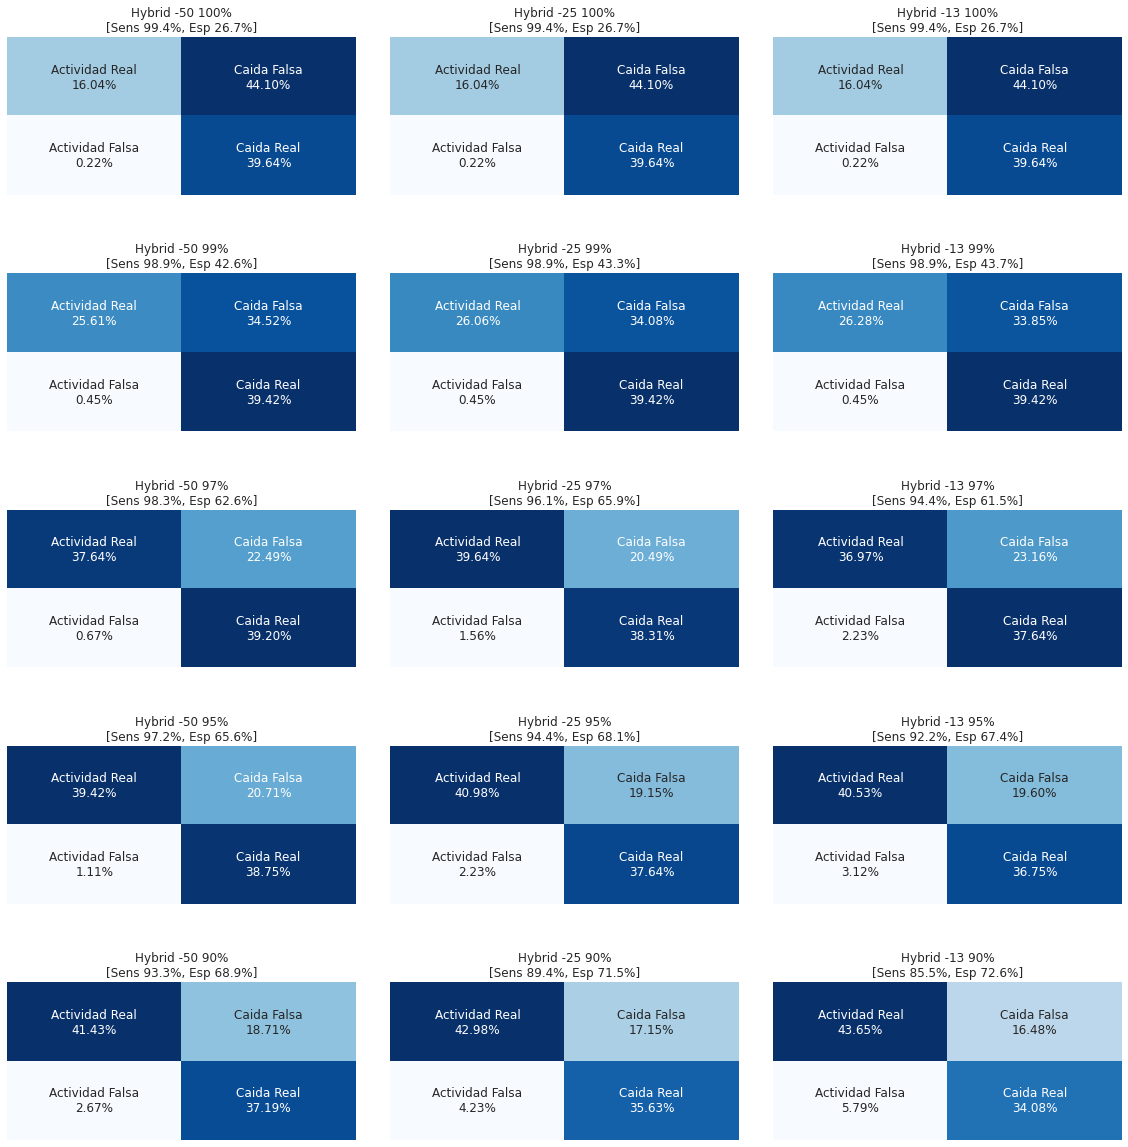
\includegraphics[width=\linewidth]{ConfMatrixRecon.png}
      \caption{\footnotesize \label{fig:ifell:adata:confmat:recon}Matrices de confusión para un modelo de reconstrucción}
  \end{subfigure}
  \hfill
  \begin{subfigure}[b]{0.45\textwidth}
      \centering
      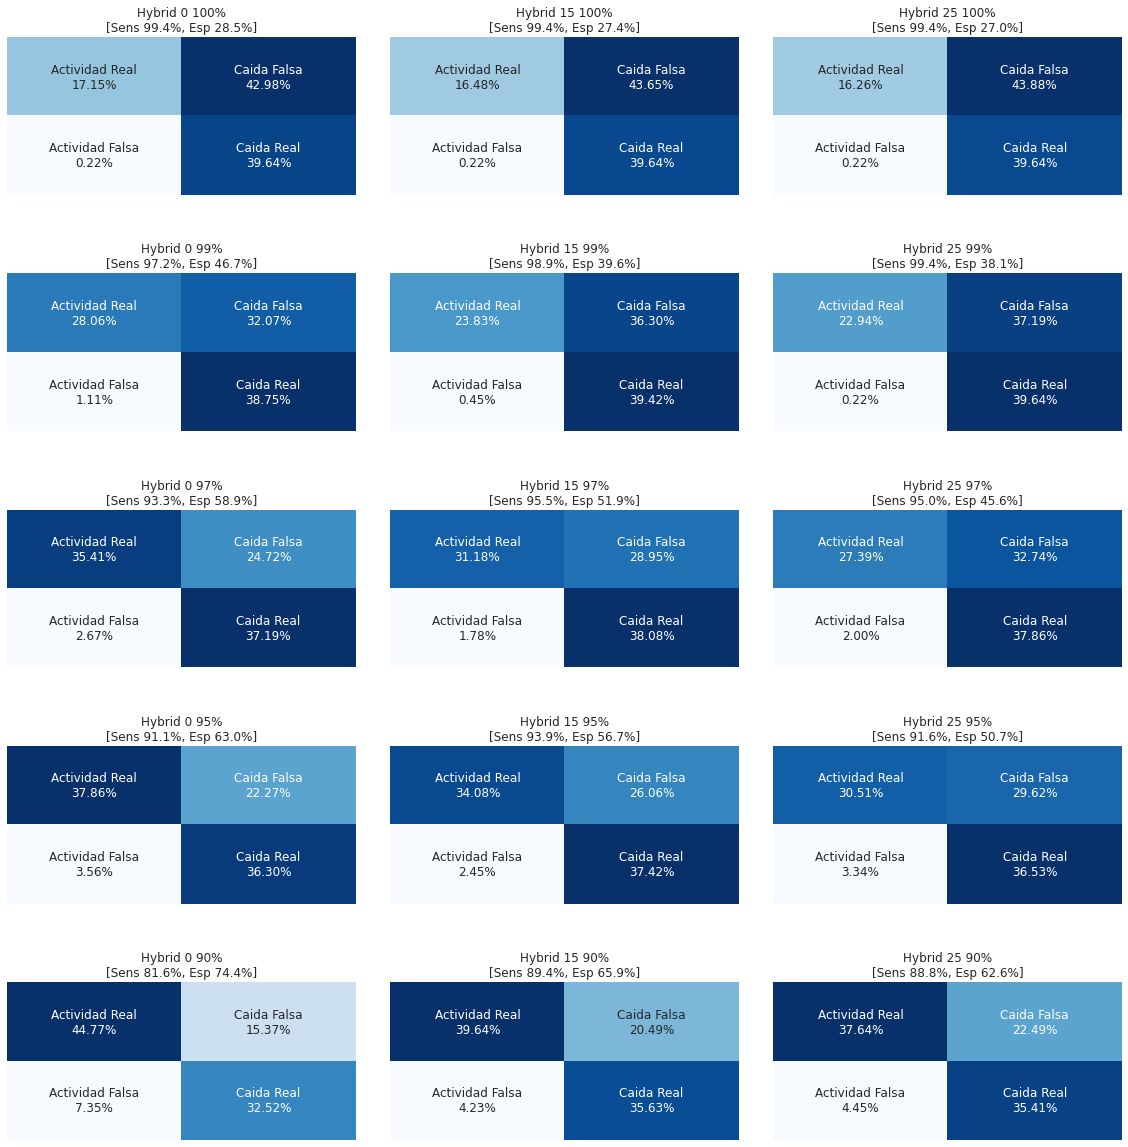
\includegraphics[width=\linewidth]{ConfMatrixPred.png}
      \caption{\footnotesize \label{fig:ifell:adata:confmat:pred}Matrices de confusión para un modelo de predicción}
  \end{subfigure}
  \caption{\label{fig:ifell:adata:confmats}Ejemplos de matrices de confusión según sensibilidad deseada y posición de la ventana}
\end{sidewaysfigure}


\begin{figure}[!ht]
  \centering
  \begin{subfigure}[b]{0.45\textwidth}
      \centering
      \includegraphics[width=\linewidth]{ADATA_RECON_RMSE_HIST}
      \caption{\footnotesize \label{fig:ifell:adata:rmshist:recon}Distribuciones de RMSE para actividades y caídas en el modelo de reconstrucción}
  \end{subfigure}
  \hfill
  \begin{subfigure}[b]{0.45\textwidth}
      \centering
      \includegraphics[width=\linewidth]{ADATA_PRED_RMS_HIST}
      \caption{\footnotesize \label{fig:ifell:adata:rmshist:pred}Distribuciones de RMSE para actividades y caídas en el modelo predicción}
  \end{subfigure}
  \caption{\label{fig:ifell:adata:rmshist}Histogramas del RMSE para los modelos IFELL}
\end{figure}

En la tabla \ref{tab:MLResults} destacan los resultados obtenidos por los modelos que usan técnicas de aprendizaje automático. Si bien en lo referente a la latencia, \cite{Liu2020} obtiene tiempos que superan el segundo en la mayoría de modelos, llegando incluso a los 8,87s obtenidos con un clasificador de Bayes. Tanto en los trabajos de \cite{Liu2018, Liu2020} como \cite{Musci2020} y \cite{Torti2018} se subraya el hecho de la no uniformidad de los resultados. Los mejores resultados se obtienen con población joven mientras que con población adulta las métricas pueden perder hasta 5 puntos, en parte debido a la falta de datos de entrenamiento. En la tabla \ref{tab:eval:resultados} se muestran los resultados de este estudio junto con los arriba mencionados y los propios resultados del estudio de \sisfall/\cite{Sucerquia2017}. Existe también el trabajo de \citeA{Putra2017} pero en su publicación no ofrece datos suficientes para obtener las métricas de especificidad, aunque clama una sensibilidad del 99,9\%. Salvo los estudios de Musci y Torti, el resto de los modelos se ejecutan en grandes equipos. Es obvio que el clasificador obtenido no alcanza la exactitud de los mejores modelos de aprendizaje automático, aunque se muestra superior a Bayes. Muestra sin embargo mejores estadísticas que los modelos analíticos sin información de la posición como Bourke y muy similar a modelos estadísticos que analizan largas secuencias. Destacamos asímismo los rápidos tiempos de ejecución de los modelos (ejecutados en los sistemas descritos en el apéndice \ref{app:colab}), un orden de magnitu mejor que el modelo CNN y dos órdenes mejor que el modelo LSTM presentados Liu. Dadas las limitaciones por los requisitos de recursos y latencia del sistema consideramos los resultados obtenidos por los clasificadores de \ifell/ satisfactorios.

% \tablas[0.80]{tab:MLResults}{Resultados de sistemas basados en ML}{lccccccccc}{
%     & \multicolumn{2}{c}{\textbf{iFell}}  & Musci2020     & Torti2018  & \multicolumn{3}{c}{Liu} &  \multicolumn{2}{\sisfall} & Bourke \\ \cmidrule{lr}{2-3}\cmidrule{lr}{4}\cmidrule{lr}{5-7}\cmidrule{lr}{8-9}
%     & Rec.  & Pred.           & LSTM & LSTM   & FD-DNN    & LSTM     & CNN   & SVM. & Best  & SVM \\ \midrule
% Sensitividad (\%) & 97,2  & 94,4          &   96,53   & 98,73       & 94,09     & 81,47   & 87,50 & \~99,99 &\~99,99  & 99,4 \\
% Especificidad (\%)& 65,6  & 63,0          &    96,01  & 97,93       & 99,94     & 99,57   & 99,88 & 32,97 & 67,97     & 29,7 \\
% Exactitud (\%)    &       &               &           & 98,33       & 99,17     & 96,88   & 98,13 & 66,43 & 83,96     & \\
% Exactitud Prom(\%)& 81,4  &               &    96,27  & 98,33       & 96,63     & 90,52   & 98,13 &       &           & 64,55\\
% Tiempo(s)         & 0,065 & 0,060         &           &             & 1,05      & 3,87    & 0,65  &  0    &           & 0\\
% }{3}

\tablan{tab:eval:resultados}{Métricas de detectores de caídas usando \sisfall/}{llccccc}{
  \emph{Estudio} & \emph{Modelo} & \emph{Sens}. & \emph{Especif.} & \emph{Exactitud} & \emph{Exact. Pond.} & \emph{Tiempo (s)} \\ \midrule
  \multirow{5}{*}{\ifell/} & RNN-R(175)[50] & 97,2  & 65,6  &     & 81,4 & 0,035 \\ 
                           & RNN-P(175)[50] & 94,4  & 63,0  &     & 78,7 & 0,031 \\
                           & IFELL-R(175)[50] & 97,8 & 65,6 &     & 82,2 & 0,035 \\
                           & IFELL-P(175)[50] & 90,5 & 68,9 &     & 79,7 & 0,031 \\
                           & Bourke & 99,4 & 29,7 &  & 64,5 & 0,0\\ \midrule[0.1]
    Musci2020                 & LSTM            & 96,5  & 96,0  &     & 92,7 & \\ \midrule[0.1]
    Torti2018                 & LSTM            & 98,7  & 97,9  & 98,3& 98,3 & \\\midrule[0.1]

    \multirow{5}{*}{Liu2018}  & SVML\tnote{1} & 97,2   & 93,6  & 95,4& 95,4 & \\
                              & SVMRBF\tnote{2} & 98,3 & 96,2 & 97,6 & 97,2 & \\
                              & kNN3   & 96,4 & 96,3 & 96,4 & 96,3 & \\
                              & Bayes  & 54,3 & 92,0 & 73,7 & 73,1 & \\
                              & DT\tnote{3} & 94,9 & 95,5 & 95,2 & 95,2 & \\\midrule[0.1]

    \multirow{3}{*}{Liu2020} & FD-DNN\tnote{4} & 94,1 & 99,9 & 99,1 & 97,0 & 1,05 \\
                             & LSTM & 81,4 & 99,5 & 96,88 & 90,4 & 3,87 \\
                             & CNN & 87,5 & 99,9 & 98,1 & 93,7 & 0,65 \\
                             & Bayes & 95,6 & 99,9 & 90,1 & 97,7 & 8,87 \\
                             & RT\tnote{5} & 92,2 & 98,5 & 80,32 & 95,3  & 1,21 \\ \midrule[0.1]

    \multirow{2}{*}{\sisfall/} & NormAcc\tnote{6} & \~99,9 & 32,97 & 66,4 & 66,4 & \\
                               & STDEV\tnote{7} & \~99,9 & 67,97 & 83,96 & 83,96 & \\
}{
\item [1] SVM Linear 
\item [2] SVM Radial Basis Function
\item [3] Decission Trees
\item [4] Deep Neural Network for Fall Detection
\item [5] Random Trees
\item [6] Norma de la aceleración en plano horizontal
\item [7] Desviación estándar del módulo
}{21}

\figura{CompositeFallNormalRMSHistogram_t-25}{fig:GRU_predictionRMS_Histogram}{Histograma de los errores de predicción del modelo GRU}

\paragraph{\ifell/ respecto a Bourke}\\
El comparador de Bourke es usado por nuestro algoritmo a modo de generador de eventos. Es además un referente en los modelos analíticos que usan el módulo de la aceleración por lo que es adecuado analizar el algoritmo de \ifell/ contra el modelo de Bourke ya que nos indicará el grado de mejora debido al desarrollo realizado. Tomaremos la variante que analiza únicamente los picos de la aceleración pues el que ha mostrado mejor comportamiento. Si forzamos una alta sensibilidad tal que $Sensibilidad \geq 99\%$ los resultados muestran una clara mejoría en la capacidad selectiva del algoritmo híbrido de \ifell/ de reconstrucción respecto al modelo de Bourke del 41\%. 

  \tablas{tab:ifell:vs:bourke}{Especificidad por modelos forzando $Sensibilidad \geq 99\%$}{lrr}{
    \emph{Modelo}     & \emph{Sensibilidad} & \emph{Especificidad} \\ \midrule
    Bourke U          & 99,0\%    & 41,3 \% \\                
    IFELL-R(175)[50]    & 99,0\%  & 58,5 \% \\
    IFELL-P(175)[50]    & 99,0\%  & 48,9 \% \\
  }{2}

\section{Evaluación de la aplicación \ifell/}

  Finalmente debemos evaluar la implementación del sistema. Partiendo del algoritmo de \ifell/ descrito en en \fullref{sec:imp:model}, e implementado en la aplicación \ifell/ usaremos un detector \textit{BourkeU} con cota de decisión en 5g como modelo analítico y los modelos \textit{IFELL-R(175)[50]} e \textit{IFELL-P(175)[50]} con cotas de decisión sobre RMSE fijadas a $RMSE_{Pred}=2,2176$ y $RMSE_{Recon}=0,2822$, es decir, buscando conseguir el 95\% de sensibilidad.

\subsection{Latencia}
    La aplicación con la configuración descrita se ha probado en un sujeto durante un periodo de dos meses de uso continuo sin pausas más allá de los periodos de carga del dispositivo. En todo este periodo no se ha producido ninguna caída real y 12 falsos positivos, la ausencia de casos positivos reales no permite realizar un análisis estadístico. Si que podemos estudiar las latencias o tiempos de ejecución del modelo recogidos en la tabla \ref{tab:ifell:watch:latencia}. Para ello medimos el tiempo desde que se invoca la petición al modelo hasta que obtenemos el resultado del comparador del nivel de decisión RMSE. 

    \tablas{tab:ifell:watch:latencia}{Tiempo de cómputo de \ifell/ en el dispositivo Fossil Sport Gen.3}{lrr}{
        \textit{Modelo}  & \textit{Float16} & \textit{Dinámico} \\ \midrule
        IFELL-P(175)[50] & 2,785 s   & 1,206 s \\
        IFELL-R(175)[50] & 2,538 s   & 1,303 s \\
        IFELL-R(350)[50] & 5,185 s   & 2,826 s \\
      }{2}

      Se aprecia el interés en optimizar los modelos para su ejecución en dispositivos embebidos. Al ser un dispositivo con una unidad GPU de capacidad limitada es la optimización a enteros don rango dinámico la que ofrece mejor tiempo de respuesta. Es notable haber conseguido unos tiempos de respuesta cercanos al segundo en un dispositivo llevable cuando tal y como se recoge en la tabla \ref{tab:eval:resultados} algunos de los modelos comparados necesitan siete veces más tiempo en un potente sistema de sobremesa. 

\subsection{Adecuación de la solución}
El objetivo de todo modelo de detección de eventos es lograr un sistema que consiga capturar la totalidad de las realizaciones del mismo con el menos número posible de falsos positivos. En otras palabras, buscamos un sistema con una especificidad y sensibilidad de 100\%\cite{Noury2007}. En el caso del sistema \ifell/ hemos optado por un enfoque que prime la facilidad de uso y sensibilidad por encima de otros aspectos. Es decir, dada una experiencia de usuario desarrollamos una aplicación que maximizase la capacidad de detección de caídas.

\subsubsection{Público objetivo}
Para definir la experiencia de usuario primero analizamos quién era el usuario objetivo. Como se ha mencionado en la introducción del trabajo, los daños relacionados con las caídas son una de las principales causas de mortaldad entre las personas mayores de 65 años. Es propio de este grupo de población la desafección por la tecnología y la carencia o desinterés por su uso. Esta condición ha de ser tenida en cuenta para el desarrollo de cualquier producto.

Las personas de edad avanzada suelen padecer así mismo de otras condiciones que pueden limitar su grado de movilidad, atención o memoria que impidan o reduzcan la posibilidad de adaptarse o incorporar nuevas rutinas. Los problemas motores y de percepción reducen notablemente la capacidad de mostrar información así como de interactuar con el usuario cuando se necesite una acción por su parte.

Se entiende por tanto que si se ha de realizar un producto para esta población, es requisito que sea lo menos obtrusivo posible, siendo recomendable incorporar la funcionalidad a un objeto de uso cotidiano para evitar la modificación de rutinas o la reticencia a incorporar nuevos procesos o elementos en su vida diaria. La interfaz de usuario debe ser mínima, usando un lenguaje visual que resulte familiar alejado de los estándares de las aplicaciones modernas. Así mismo, reducir o eliminar los procesos de configuración y manipulación, con un sistema que funcione desde la primera ejecución.

\subsubsection{Plataforma y localización}
Teniendo en cuenta los requisitos anteriores optamos por un objeto vestible de uso cotidiano. Un complemento al que el usuario esté acostumbrado que sería reemplazado por el sistema desarrollado. Optamos por desarrollar el sistema sobre un reloj inteligente. Este objeto se asemeja en forma y función a los tradicionales relojes mecánicos y automáticos a los que la población adulta les resulta familiar y conocido. La recarga de la batería, único punto diferencial con respecto a los relojes tradicionales, no dista mucho de la necesidad de remontar el mecanismo de reserva de energía mecánica de sus homólogos no computerizados.

Esta decisión es la que tendrá mayor impacto sobre la funcionalidad del prototipo ya que fuerza la posición del dispositivo de captura. Diversos estudios muestran que el mejor lugar para posicionar un sistema de medición de la aceleración para detectar caídas es la cintura, seguida de la cabeza siendo desaconsejado usar sensores en las extremidades por su alta movilidad\cite{Chen2005, Kangas2008, Noury2007}. Al usar un reloj, y por tanto posicionar los sensores en la muñeca no sólo estamos penalizando la calidad de las lecturas sino que reducimos la capacidad de obtener información de la actitud o postura del cuerpo. Esta información permite desarrollar índices de detección analíticos de muy alta calidad, sin embargo por la posición tendremos que usar métodos basados únicamente en la norma del vector aceleración.

A juicio del autor, la penalización cualitativa resultante de dicha decisión queda compensada por la usabilidad de la plataforma. El mejor de los detectores de caídas resulta inútil si el usuario no lo utiliza. A este respecto, ninguno de los sujetos del ensayo tuvo problema alguno para manipular el sistema, a pesar de ser una muestra demasiado reducida para ser significativa.

\subsubsection{Interfaz y autonomía}
\figura{appBatt}{fig:ifell:bateria}{Consumo de batería}
La necesidad de interacción del usuario con el sistema es mínima y siempre opcional. Instalar la aplicación significa configurar una determinado aspecto de la esfera del reloj que presenta un aspecto analógico tradicional con manecillas para indicar horas, minutos y segundos y un pequeño mensaje de estado. Esta opción garantiza que el propio sistema operativo lanzará la aplicación tras cada arranque. A su vez los servicios necesarios se ejecutan siempre en segundo plano de manera que incluso si se usa otra aplicación en el dispositivo la detección de caídas sigue en marcha. Las única manipulación necesaria con el objeto es el proceso de carga. Con el fin de maximizar el tiempo entre cargas y con la meta de conseguir al menos 24 horas de autonomía se optó por un enfoque de modelo híbrido. En la \autoref{fig:ifell:bateria} se mostramos una captura de la pantalla de gestión de la batería del sistema operativo del reloj tras un día de uso con \ifell/ ejecutándose. Es un caso extremo ya que durante ese periodo no no se usó el reloj ni se encendió la pantalla en ningún momento. Sin embargo muestra que es fácil mantener 24 horas de actividad entre cargas sin problema. Este resultado es una clara mejoría con respecto a los experimentos previos como \citeA{Liu2020} en que el módulo de captura únicamente tiene una duración de 30 horas en envío de datos a la unidad de proceso, o las 20 horas de la unidad llevable que auna cómputo y medición propuesta por \citeA{Torti2018}. Confirmamos que la elección del algoritmo híbrido de detección ha resultado instrumental en conseguir modelos de muy alta eficiencia energética.


